% Source : 

\documentclass{standalone}
 
\usepackage{tikz}
\usetikzlibrary{arrows,positioning, calc} 
\tikzstyle{vertex}=[draw,fill=black!15,circle,minimum size=20pt,inner sep=0pt]


\begin{document}
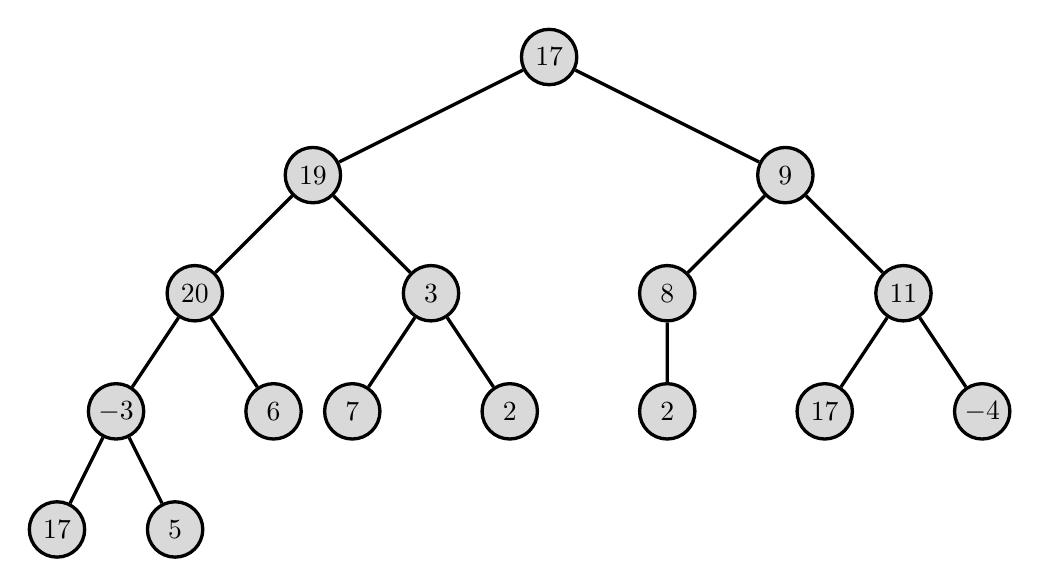
\begin{tikzpicture}[very thick,level/.style={sibling distance=60mm/#1}]
\node [vertex] (r){$17$}
  child {
    node [vertex] (a) {$19$}
    child {
      node [vertex] {$20$}
      child {
        node [vertex] {$-3$}
        child {node [vertex] {$17$}}
        child {node [vertex] {$5$}}
      } 
      child {node [vertex] {$6$}}
    }
    child {
      node [vertex] {$3$}
      child {node [vertex] {$7$}}
      child {node [vertex] {$2$}}
    }
  }
  child {
    node [vertex] {$9$}
    child {
      node [vertex] {$8$}
      child {node [vertex] {$2$}}
    }
    child {
      node [vertex] {$11$}
      child {node [vertex] {$17$}}
      child {node [vertex] {$-4$}}
    }
  };
\end{tikzpicture}
\end{document}